\documentclass[%
autoref,     % тип документа
%natbib,      % использовать пакет natbib для "сжатия" цитирований
href,        % использовать пакет hyperref для создания гиперссылок
colorlinks,  % цветные гиперссылки
%times,      % шрифт Times как основной
%fixint,     % включить прямые знаки интегралов
%classified, % гриф секретности
%facsimile,   % отображать факсимиле диссертанта и ученого секретаря
]{disser}

\usepackage[
  a4paper, mag=1000,
  left=2.5cm, right=1cm, top=2cm, bottom=2cm, headsep=0.7cm, footskip=1cm
]{geometry}

\usepackage[intlimits]{amsmath}
\usepackage{amssymb,amsfonts}
\usepackage[autostyle]{csquotes}

\usepackage[T2A]{fontenc}
\usepackage[utf8]{inputenc}
\usepackage[english,russian]{babel}
\usepackage{tabularx}
\ifpdf\usepackage{epstopdf}\fi

\usepackage[
style=gost-numeric,
backend=biber,
autolang=other,
sorting=nyt,
bibencoding=utf8,
maxbibnames=1,
minbibnames=1,
doi=false,
isbn=false,
defernumbers=true
]{biblatex}

\addbibresource{thesis.bib}

% Номера страниц снизу и по центру
\pagestyle{footcenter}
\chapterpagestyle{footcenter}

% Точка с запятой в качестве разделителя между номерами цитирований
%\setcitestyle{semicolon}

% Путь к файлам с иллюстрациями
\graphicspath{{fig/}}

\begin{document}
% Включение файла с общим текстом диссертации и автореферата
% (текст титульного листа и характеристика работы).
% Общие поля титульного листа диссертации и автореферата
\institution{
	Федеральный исследовательский центр <<Информатика и Управление>> Российской академии наук \\
	ФИЦ ИУ РАН}

\topic{Методы и алгоритмы биометрического распознавания человека по радужной оболочке глаза на мобильном устройстве}

\author{Одиноких Глеб Андреевич}

\specnum{05.13.17}
\spec{Теоретические основы информатики}

\sa{Матвеев Иван Алексеевич}
\sastatus{д.~т.~н.}
%\sasnd{ФИО второго руководителя}
%\sasndstatus{к.~ф.-м.~н., проф.}

%\scon{ФИО консультанта}
%\sconstatus{д.~ф.-м.~н., проф.}
%\sconsnd{ФИО второго консультанта}
%\sconsndstatus{д.~ф.-м.~н., проф.}

\begin{picture}(50,50)
\put(350,-200){\hbox{\includegraphics[scale=0.25]{pictures/sign_Odinokikh.png}}}
\end{picture}

\city{Москва}
\date{\number\year}

% Общие разделы автореферата и диссертации
\mkcommonsect{actuality}{Актуальность темы исследования}{%
В попытках изобрести надёжные и при этом удобные способы подтверждения подлинности той или иной информации, общество проделало огромный путь от парольных фраз, сложных печатей, механических замков и ключей до методов автоматической аутентификации. Подтверждение личности при пересечении границ регионов и государств, приобретении товаров и услуг, попытках доступа к различного рода данным и устройствам, проведении всевозможных финансовых транзакций, сопровождающиеся необходимостью предоставления подтверждающей информации, становится регулярной и неотъемлемой частью жизни каждого. Более 522 млрд. безналичных платёжных транзакций было произведено в 2017 году, 282 и 389 млрд. в 2010 и 2014 годах соответственно, согласно World Payments Report 2017 (WPR2017)~\cite{wpr_2017}, а прогнозируемое к 2020 году значение может достигнуть 726 млрд. Количество безналичных платёжных операций стремительно увеличивается, вместе с ним растёт и доля операций, совершенная при помощи мобильных устройств. По данным WPR2017 в период с 2015-2019 гг. ожидаемый рост доли транзакций, осуществляемых с их помощью, составит 21.8\% и 32\% в период 2017-2022 гг. Каждая транзакция, проводимая при помощи мобильного устройства, требует предоставления подтверждающей информации (ПИН-код и др.). Помимо транзакций, требующих непосредственного участия пользователя, существует устойчивый тренд к персонификации и интеллектуализации различных сервисов и услуг, среди которых т.н. <<умный дом>> (Smart Home), интернет вещей (Internet of Things), роботы-помощники (Smart Assistant и др.) и многое другое. Здесь речь может идти и о т.н. некооперативном распознавании. Практически каждое из вышеперечисленных приложений подразумевает наличие системы автоматической аутентификации/идентификации пользователя.

Развитие систем компьютерного зрения, машинного (в особенности глубокого) обучения, регистрации и обработки цифровых изображений, распознавания образов в совокупности увеличением мощности вычислительных устройств, позволили совершить значительный рывок в области \textit{биометрической идентификации} личности. В качестве идентификатора здесь выступает уникальная \textit{биометрическая характеристика человека (БХЧ)} или \textit{биометрическая модальность}. К числу наиболее часто используемых для распознавания БХЧ можно отнести следующие: изображение и форма лица, изображения радужной оболочки, сетчатки и периокулярной области глаза, папиллярный узор пальцев и ладони, изображение венозного русла кисти и ладони, особенности голоса, почерка, походки. Изображение радужки, обладающей сложной структурой, индивидуальной для каждого человека, является богатым источником информации. Биометрические системы, использующие изображение РОГ в качестве биометрической модальности, на сегодняшний день показывают наивысшую точность распознавания, и поэтому привлекают внимание множества исследователей по всему миру.

Среди наиболее известных исследовательских групп: Cambridge University, Великобритания (J. Daugman); Michigan State University, США (J. Anil, A. Ross); University of Notre Dame, США (P.J. Flynn, K.W. Bowyer), University of Beira Interior, Португалия (H. Proenca), Warsaw University of Technology, Польша (A. Czajka), Institute of Automation of the Chinese Academy of Sciences, КНР (T. Tan), в том числе и несколько российских: Федеральный Исследовательский центр <<Информатика и управление>> РАН (д.т.н. И.А. Матвеев), МГУ им. Ломоносова (д.ф-м.н. А.С. Крылов), Институт систем обработки изображений РАН и др. Тем не менее, наибольшее внимание технологиям биометрического распознавания сейчас уделяется со стороны коммерческих компаний, создающих целые институты и направления для их реализации и доведения до рынка.

Использование биометрических технологий в мобильных устройствах и в системах некооперативного распознавания подразумевает удобство их использования, быстродействие и устойчивость к изменчивости БХЧ и окружения. Это вынуждает ужесточать требования как к алгоритмам распознавания, так и к средствам регистрации изображения. В частности, система должна осуществлять устойчивое извлечение биометрического признака(-ов) из изображения низкого качества, его обработку и последующее сравнение в режиме реального времени, обеспечивая при этом низкие значения ошибки ложного недопуска \textit{(False Rejection Rate - FRR)}. Биометрический шаблон должен быть защищен. Защита может осуществляться на системном уровне и добавлением спецальных алгоритмов хеширования биометрических данных. Кроме этого, к основным требованиям часто относят необходимость взаимодействия с пользователем и наличие системы защиты от подделки. Весь процесс обработки должен осуществляться на устройстве с сильно ограниченными вычислительными ресурсами.

Таким образом, новые сценарии использования технологий биометрического распознавания создают новые задачи, решение которых позволит существенно повысить уровень безопасности и удобства транзакций, ежедневно осущещствляемых миллионами людей по всему миру, при использовании различных сервисов и услуг.

Наиболее актуальными направлениями развития области распознавания по РОГ на сегодняшний день являются: оценка качества изображения радужки в условиях изменчивости окружения и при некооперативном распознавании; разработка методов сегментации области радужки на изображении низкого качества; разработка высокопроизводительных методов извлечения и представления особенностей радужки из изображения низкого качества; анализ информативных признаков радужки и периокулярной области глаза с целью обеспечения обратной связи с пользователем; создание устойчивых методов сравнения биометрических шаблонов радужки, получаемых в условиях значительной изменчивости окружения; разработка новых методов защиты от подделки.
}

\mkcommonsect{development}{Степень разработанности темы исследования.}{
Текст о степени разработанности темы.
}

\mkcommonsect{objective}{Цели и задачи диссертационной работы:}{%

В работе были поставлены следующие \textbf{цели}:

\begin{itemize}
	\item[$\bullet$] Создать методы и алгоритмы для автоматического распознавания человека по радужной оболочке глаза, способные обрабатывать изображение радужки с частотой поступления кадров на мобильном устройстве, удовлетворяющие критериям ошибок распознавания:  $FRR\leq1\%$ при $FAR<10^{-7}$
	\item[$\bullet$] Разработать методы и алгоритмы оценки качества изображения радужки, определяющие её пригодность для выделения признаков и обеспечивающие обратную связь с пользователем устройства
	\item[$\bullet$] Разработать методы и алгоритмы выделения области радужки на изображении низкого качества
	\item[$\bullet$] Создать методы и алгоритмы выявления подделок радужки по изображению низкого качества, способный обеспечивать защиту от ранее не рсмматриваемых видов атак
\end{itemize}

Для достижения поставленных целей были решены следующие \textbf{задачи}:

\begin{itemize}
	\item[$\bullet$] Исследование и разработка методов распознавания человека по радужке, удовлетворяющих критериям, необходимым для обеспечения возможности их применения в мобильном устройстве
	\item[$\bullet$] Разработка метода оценки качества изображения радужки, учитывающего ограничения, особенности использования мобильного устройства и взаимодействия c пользователем
	\item[$\bullet$] Исследование и разработка методов выделения радужки на изображении низкого качества, получаемого в условиях постоянно изменяющегося окружения
	\item[$\bullet$] Исследование и разработка методов извлечения и сравнения уникальных особенностей радужки из изображения низкого качества в условиях постоянно изменяющегося окружения
	\item[$\bullet$] Исследование и разработка методов обнаружения попыток представления подделок радужной оболочки глаза
	\item[$\bullet$] Сбор и разметка баз данных изображений для проведения экспериментов в рамках решения вышеперечисленных задач
	\item[$\bullet$] Создание среды и программных средств для оценки производительности методов, реализованных в рамках решения вышеперечисленных задач
	\item[$\bullet$] Создание программных средств (библиотеки и демо-приложений) для апробации реализованных методов на мобильном устройстве
\end{itemize}
}

\mkcommonsect{novelty}{Научная новизна.}{%
\begin{itemize}
	\item[$\bullet$] Предложен новый высокопроизводительный метод распознавания человека по радужной оболочке глаза, способный работать на устройстве с низкой вычислительной мощностью в условиях постоянно изменяющегося окружения в режиме реального времени;
	\item[$\bullet$] Предложен новый высокопроизводительный метод выделения области радужки на изображении низкого качества;
	\item[$\bullet$] Разработан новый метод оценки качества изображения радужки, позволяющий оценить её пригодностьдля извлечения уникальных особенностей и их последующего сравнения, обеспечивающий обратную связь с пользователем в виде отображения подсказок на экране устройства;
	\item[$\bullet$] Разработан новый метод адаптивного квантования изображения радужки, устойчивый к искажениям текстуры радужки;
	\item[$\bullet$] Предложен новый метод извлечения и сравнения уникальных особенностей радужки, обеспечивающий высокую точность распознавания, устойчивый к изменению размера зрачка, условий окружения и уровню качества изображения;
	\item[$\bullet$] Разработан новый надежный метод защиты от подделывания радужки, обеспечивающий защиту от, в том числе, ранее не рассматриваемых видов атак;
\end{itemize}
}

\mkcommonsect{value}{Теоретическая и практическая значимость.}{%
Результаты, изложенные в диссертации, используются в мобильных устройствах, выпускаемых компанией Samsung Electronics Co. Ltd. Среди устройств флагманские модели, выпускаемые компанией в период с 2016 по 2018 гг.: смартфон Samsung Galaxy Note7, смартфоны Samsung Galaxy S8/S8+, смартфон Samsung Galaxy Note8, смартфоны Samsung Galaxy S9/S9+, смартфон Samsung Galaxy Note9, планшет Samsung Galaxy Tab S4.
}

\mkcommonsect{methods}{Методология и методы исследования.}{%
Текст о методах исследования.
}

\mkcommonsect{results}{Положения, выносимые на защиту:}{
	
\begin{itemize}
	\item[$\bullet$] Исследованы особенности использования методов биометрического распознавания человека по радужной оболочке глаза в применении к мобильным устройствам, сформулированы основные требования, предъявляемые к таким методам;
	\item[$\bullet$] Разработан метод распознавания пользователя смартфона по изображению радужной оболочки глаза, собрана база данных изображений радужки, полученных в условиях, симулирующих реальное взаимодействие пользователя с устройством при распознавании, осуществлена программная реализация метода, произведено сравнение с аналогами, известными из литературы, по точности и скорости распознавания;
	\item[$\bullet$] Предложен многостадийный метод оценки качества изображения радужки, получаемого при помощи мобильного устройства, позволяющий обеспечивать обратную связь с пользователем в виде отображения подсказок на экране устройства;
	\item[$\bullet$] Исследованы методы выделения области радужки на изображении, получаемом в экстремальных условиях окружения, разработан и программно реализован метод, основанный на глубоком обучении, произведена его оценка и сравнение с известными из литературы аналогами;
	\item[$\bullet$] Исследованы, разработаны и программно реализованы методы извлечения уникальных особенностей радужки по изображению, получаемому в экстремальных условиях окружения, произведено сравнение методов с существующими аналогами по скорости обработки и точности распознавания;
	\item[$\bullet$] 6.	Исследованы новые виды подделок радужки, собрана база данных подделок, предложен метод защиты от подделок, устойчивый к новым видам подделок, произведено его сравнение с известными из литературы методами по точности детектирования и скорости обработки.
\end{itemize}

}

\mkcommonsect{approbation}{Степень достоверности и апробация результатов.}{%
Достоверность результатов обеспечивается обширным анализом работ в области исследования, описанием проведенных экспериментов, их воспроизводимостью, а так же апробацией результатов на практике.
Основные результаты диссертации докладывались на следующих конференциях: The 12th IAPR International Conference On Biometrics, Crete, Greece, 2019; International Conference on Pattern Recognition and Artificial Intelligence, Montreal, Canada, 2018; International Workshop on "Photogrammetric and computer vision techniques for video surveillance, biometrics and biomedicine", Moscow, Russia, 2017; Intelligent Data Processing Conference, Barcelona, Spain, 2016; Intelligent Data Processing Conference, Gaeta, Italy 2018; Samsung Mobile Developers Conference, Suwon, 2016, South Korea; Всероссийская научная конференции ЭКОМОД-2016, Киров, Россия, 2016.

}

\mkcommonsect{pub}{Публикации.}{%
Материалы диссертации опубликованы в $10$ печатных работах, из них 3 в журналах из списка ВАК.
}

\mkcommonsect{contrib}{Личный вклад автора.}{%
Содержание диссертации и основные положения, выносимые на защиту, отражают персональный вклад автора в опубликованные работы.
Подготовка к публикации полученных результатов проводилась совместно с соавторами, причем вклад диссертанта был определяющим. Все представленные в диссертации результаты получены лично автором.
}

\mkcommonsect{struct}{Структура и объем диссертации.}{%
Диссертация состоит из введения, обзора литературы, 5 глав, заключения и библиографии.
Общий объем диссертации 106 страниц, из них 88 страниц текста, включая 34 рисунков.
Библиография включает 154 наименований на 17 страницах.
}


% номер копии для грифа секретности
%\copynum{1}
% класс доступа
%\classlabel{Для служебного пользования}

\title{АВТОРЕФЕРАТ\\
диссертации на соискание ученой степени\\
кандидата технических наук}

\maketitle

% Внутренняя сторона обложки
\thispagestyle{empty}
\vspace*{-2cm}
\noindent
\begin{center}
Работа выполнена в \emph{Федеральный исследовательский центр <<Информатика и Управление>> Российской академии наук (ФИЦ ИУ РАН)}.
\end{center}
\vskip1ex\noindent
\begin{tabularx}{\linewidth}{@{}lX@{}}
  \textbf{Научный руководитель:} & \textbf{Матвеев Иван Алексеевич}\\
  & доктор технических наук, главный научный сотрудник отдела № 31 Федерального исследовательского центра <<Информатика и управление>> Российской академии наук \\[6pt]
  \textbf{Официальные оппоненты:} & \textbf{Гостев Иван Михайлович}\\
  & доктор технических наук, профессор ФГАОУ ВО <<Национальный исследовательский университет <<Высшая школа экономики>>\\[6pt]
  & \textbf{Трёкин Алексей Николаевич}\\
  & кандидат технических наук, научный сотрудник <<Центра по научным и инженерным вычислительным технологиям для задач с большими массивами данных>> Сколковского института науки и технологий\\[6pt]
  \textbf{Ведущая организация:} & ФГБОУ ВО «Московский Государственный Университет имени М.В. Ломоносова»
\end{tabularx}

\vskip2ex\noindent
Защита состоится \datefield{} в \rule[0pt]{1cm}{0.5pt} часов
на заседании диссертационного совета Д 002.073.05 при Федеральном исследовательском центре «Информатика и управление» Российской академии наук (ФИЦ ИУ РАН) по адресу 119333, г. Москва, ул. Вавилова, д. 40.

\vskip1ex\noindent
С диссертацией можно ознакомиться в библиотеке и на сайте ФИЦ ИУ РАН http://frccsc.ru.

\vskip1ex\noindent
Автореферат разослан \datefield{}

\vskip1ex\noindent
\vfill\noindent
\begin{minipage}[b]{0.5\linewidth}
  Ученый секретарь\\
  диссертационного совета Д 002.073.05, \\
  д.ф.-м.н., профессор
\end{minipage}
\hfill
% вставка файла, содержащего факсимиле ученого секретаря
\makeatletter
%\ifDis@facsimile
%  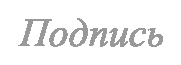
\includegraphics[width=3cm]{sec-facsimile}\hfill
%\fi%
\makeatother%
\emph{Рязанов В.В.}

%\clearpage
%
%\nsection{Общая характеристика работы}
%
%% Актуальность работы
%\actualitysection
%\actualitytext
%
%% Степень разработанности темы исследования
%\developmentsection
%\developmenttext
%
%% Цели и задачи диссертационной работы
%\objectivesection
%\objectivetext
%
%% Научная новизна
%\noveltysection
%\noveltytext
%
%% Теоретическая и практическая значимость
%\valuesection
%\valuetext
%
%% Методология и методы исследования
%\methodssection
%\methodstext
%
%% Положения, выносимые на защиту
%\resultssection
%\resultstext
%
%% Степень достоверности и апробация результатов
%\approbationsection
%\approbationtext
%
%% Публикации
%\pubsection
%\pubtext
%
%% Личный вклад автора
%\contribsection
%\contribtext
%
%% Структура и объем диссертации
%\structsection
%\structtext
%
%\nsection{Содержание работы}
%
%\textbf{Во Введении} обоснована актуальность диссертационной работы, сформулирована цель и аргументирована научная новизна исследований, показана практическая значимость полученных результатов, представлены выносимые на защиту научные положения.
%
%\textbf{В первой главе} ...
%
%Содержание первой главы.
%
%Результаты первой главы опубликованы в работе~\cite{Ivanov_1999_Journal_17_173}.
%
%\textbf{Во второй главе} ...
%
%Содержание второй главы.
%
%Результаты второй главы опубликованы в работе~\cite{Petrov_2001_Journal_23_12321}.
%
%\textbf{В третьей главе} ...
%
%Содержание третьей главы.
%
%Результаты третьей главы опубликованы в работе~\cite{Sidorov_2002_Journal_32_1531}.
%
%\textbf{В Заключении}
%
%% ----------------------------------------------------------------
%\printbibliography[keyword=own,title={Основные публикации по теме диссертации}]
%\printbibliography[notkeyword=own,title={Цитированная литература}]
%
%% ----------------------------------------------------------------
%% Выходные данные
%\clearpage
%\thispagestyle{empty}
%\normalfont\selectfont
%\vspace*{2cm}
%\begin{center}
%\textit{Научное издание}\\
%\vskip 2cm
%\makeatletter
%\@author
%\vskip 1.5cm
%\@title{} на тему:\\
%\@topic\\
%\makeatother
%\end{center}
%\vfill
%Подписано в печать~25.01.2011.
%Формат~$60 \times 90$~1/16.
%Тираж~100~экз.
%Заказ~256.\\[2ex]
%\noindent
%Санкт-Петербургская издательская фирма <<Наука>> РАН.
%199034, Санкт-Петербург, Менделеевская линия, 1,
%\href{http://www.naukaspb.spb.ru}{http://www.naukaspb.spb.ru}

\end{document}
